% Options for packages loaded elsewhere
% Options for packages loaded elsewhere
\PassOptionsToPackage{unicode}{hyperref}
\PassOptionsToPackage{hyphens}{url}
\PassOptionsToPackage{dvipsnames,svgnames,x11names}{xcolor}
%
\documentclass[
  11pt,
  letterpaper,
]{scrbook}
\usepackage{xcolor}
\usepackage[top=1in,bottom=1in,left=1.25in,right=1.25in]{geometry}
\usepackage{amsmath,amssymb}
\setcounter{secnumdepth}{5}
\usepackage{iftex}
\ifPDFTeX
  \usepackage[T1]{fontenc}
  \usepackage[utf8]{inputenc}
  \usepackage{textcomp} % provide euro and other symbols
\else % if luatex or xetex
  \usepackage{unicode-math} % this also loads fontspec
  \defaultfontfeatures{Scale=MatchLowercase}
  \defaultfontfeatures[\rmfamily]{Ligatures=TeX,Scale=1}
\fi
\usepackage{lmodern}
\ifPDFTeX\else
  % xetex/luatex font selection
\fi
% Use upquote if available, for straight quotes in verbatim environments
\IfFileExists{upquote.sty}{\usepackage{upquote}}{}
\IfFileExists{microtype.sty}{% use microtype if available
  \usepackage[]{microtype}
  \UseMicrotypeSet[protrusion]{basicmath} % disable protrusion for tt fonts
}{}
\makeatletter
\@ifundefined{KOMAClassName}{% if non-KOMA class
  \IfFileExists{parskip.sty}{%
    \usepackage{parskip}
  }{% else
    \setlength{\parindent}{0pt}
    \setlength{\parskip}{6pt plus 2pt minus 1pt}}
}{% if KOMA class
  \KOMAoptions{parskip=half}}
\makeatother
% Make \paragraph and \subparagraph free-standing
\makeatletter
\ifx\paragraph\undefined\else
  \let\oldparagraph\paragraph
  \renewcommand{\paragraph}{
    \@ifstar
      \xxxParagraphStar
      \xxxParagraphNoStar
  }
  \newcommand{\xxxParagraphStar}[1]{\oldparagraph*{#1}\mbox{}}
  \newcommand{\xxxParagraphNoStar}[1]{\oldparagraph{#1}\mbox{}}
\fi
\ifx\subparagraph\undefined\else
  \let\oldsubparagraph\subparagraph
  \renewcommand{\subparagraph}{
    \@ifstar
      \xxxSubParagraphStar
      \xxxSubParagraphNoStar
  }
  \newcommand{\xxxSubParagraphStar}[1]{\oldsubparagraph*{#1}\mbox{}}
  \newcommand{\xxxSubParagraphNoStar}[1]{\oldsubparagraph{#1}\mbox{}}
\fi
\makeatother

\usepackage{color}
\usepackage{fancyvrb}
\newcommand{\VerbBar}{|}
\newcommand{\VERB}{\Verb[commandchars=\\\{\}]}
\DefineVerbatimEnvironment{Highlighting}{Verbatim}{commandchars=\\\{\}}
% Add ',fontsize=\small' for more characters per line
\usepackage{framed}
\definecolor{shadecolor}{RGB}{241,243,245}
\newenvironment{Shaded}{\begin{snugshade}}{\end{snugshade}}
\newcommand{\AlertTok}[1]{\textcolor[rgb]{0.68,0.00,0.00}{#1}}
\newcommand{\AnnotationTok}[1]{\textcolor[rgb]{0.37,0.37,0.37}{#1}}
\newcommand{\AttributeTok}[1]{\textcolor[rgb]{0.40,0.45,0.13}{#1}}
\newcommand{\BaseNTok}[1]{\textcolor[rgb]{0.68,0.00,0.00}{#1}}
\newcommand{\BuiltInTok}[1]{\textcolor[rgb]{0.00,0.23,0.31}{#1}}
\newcommand{\CharTok}[1]{\textcolor[rgb]{0.13,0.47,0.30}{#1}}
\newcommand{\CommentTok}[1]{\textcolor[rgb]{0.37,0.37,0.37}{#1}}
\newcommand{\CommentVarTok}[1]{\textcolor[rgb]{0.37,0.37,0.37}{\textit{#1}}}
\newcommand{\ConstantTok}[1]{\textcolor[rgb]{0.56,0.35,0.01}{#1}}
\newcommand{\ControlFlowTok}[1]{\textcolor[rgb]{0.00,0.23,0.31}{\textbf{#1}}}
\newcommand{\DataTypeTok}[1]{\textcolor[rgb]{0.68,0.00,0.00}{#1}}
\newcommand{\DecValTok}[1]{\textcolor[rgb]{0.68,0.00,0.00}{#1}}
\newcommand{\DocumentationTok}[1]{\textcolor[rgb]{0.37,0.37,0.37}{\textit{#1}}}
\newcommand{\ErrorTok}[1]{\textcolor[rgb]{0.68,0.00,0.00}{#1}}
\newcommand{\ExtensionTok}[1]{\textcolor[rgb]{0.00,0.23,0.31}{#1}}
\newcommand{\FloatTok}[1]{\textcolor[rgb]{0.68,0.00,0.00}{#1}}
\newcommand{\FunctionTok}[1]{\textcolor[rgb]{0.28,0.35,0.67}{#1}}
\newcommand{\ImportTok}[1]{\textcolor[rgb]{0.00,0.46,0.62}{#1}}
\newcommand{\InformationTok}[1]{\textcolor[rgb]{0.37,0.37,0.37}{#1}}
\newcommand{\KeywordTok}[1]{\textcolor[rgb]{0.00,0.23,0.31}{\textbf{#1}}}
\newcommand{\NormalTok}[1]{\textcolor[rgb]{0.00,0.23,0.31}{#1}}
\newcommand{\OperatorTok}[1]{\textcolor[rgb]{0.37,0.37,0.37}{#1}}
\newcommand{\OtherTok}[1]{\textcolor[rgb]{0.00,0.23,0.31}{#1}}
\newcommand{\PreprocessorTok}[1]{\textcolor[rgb]{0.68,0.00,0.00}{#1}}
\newcommand{\RegionMarkerTok}[1]{\textcolor[rgb]{0.00,0.23,0.31}{#1}}
\newcommand{\SpecialCharTok}[1]{\textcolor[rgb]{0.37,0.37,0.37}{#1}}
\newcommand{\SpecialStringTok}[1]{\textcolor[rgb]{0.13,0.47,0.30}{#1}}
\newcommand{\StringTok}[1]{\textcolor[rgb]{0.13,0.47,0.30}{#1}}
\newcommand{\VariableTok}[1]{\textcolor[rgb]{0.07,0.07,0.07}{#1}}
\newcommand{\VerbatimStringTok}[1]{\textcolor[rgb]{0.13,0.47,0.30}{#1}}
\newcommand{\WarningTok}[1]{\textcolor[rgb]{0.37,0.37,0.37}{\textit{#1}}}

\usepackage{longtable,booktabs,array}
\usepackage{calc} % for calculating minipage widths
% Correct order of tables after \paragraph or \subparagraph
\usepackage{etoolbox}
\makeatletter
\patchcmd\longtable{\par}{\if@noskipsec\mbox{}\fi\par}{}{}
\makeatother
% Allow footnotes in longtable head/foot
\IfFileExists{footnotehyper.sty}{\usepackage{footnotehyper}}{\usepackage{footnote}}
\makesavenoteenv{longtable}
\usepackage{graphicx}
\makeatletter
\newsavebox\pandoc@box
\newcommand*\pandocbounded[1]{% scales image to fit in text height/width
  \sbox\pandoc@box{#1}%
  \Gscale@div\@tempa{\textheight}{\dimexpr\ht\pandoc@box+\dp\pandoc@box\relax}%
  \Gscale@div\@tempb{\linewidth}{\wd\pandoc@box}%
  \ifdim\@tempb\p@<\@tempa\p@\let\@tempa\@tempb\fi% select the smaller of both
  \ifdim\@tempa\p@<\p@\scalebox{\@tempa}{\usebox\pandoc@box}%
  \else\usebox{\pandoc@box}%
  \fi%
}
% Set default figure placement to htbp
\def\fps@figure{htbp}
\makeatother


% definitions for citeproc citations
\NewDocumentCommand\citeproctext{}{}
\NewDocumentCommand\citeproc{mm}{%
  \begingroup\def\citeproctext{#2}\cite{#1}\endgroup}
\makeatletter
 % allow citations to break across lines
 \let\@cite@ofmt\@firstofone
 % avoid brackets around text for \cite:
 \def\@biblabel#1{}
 \def\@cite#1#2{{#1\if@tempswa , #2\fi}}
\makeatother
\newlength{\cslhangindent}
\setlength{\cslhangindent}{1.5em}
\newlength{\csllabelwidth}
\setlength{\csllabelwidth}{3em}
\newenvironment{CSLReferences}[2] % #1 hanging-indent, #2 entry-spacing
 {\begin{list}{}{%
  \setlength{\itemindent}{0pt}
  \setlength{\leftmargin}{0pt}
  \setlength{\parsep}{0pt}
  % turn on hanging indent if param 1 is 1
  \ifodd #1
   \setlength{\leftmargin}{\cslhangindent}
   \setlength{\itemindent}{-1\cslhangindent}
  \fi
  % set entry spacing
  \setlength{\itemsep}{#2\baselineskip}}}
 {\end{list}}
\usepackage{calc}
\newcommand{\CSLBlock}[1]{\hfill\break\parbox[t]{\linewidth}{\strut\ignorespaces#1\strut}}
\newcommand{\CSLLeftMargin}[1]{\parbox[t]{\csllabelwidth}{\strut#1\strut}}
\newcommand{\CSLRightInline}[1]{\parbox[t]{\linewidth - \csllabelwidth}{\strut#1\strut}}
\newcommand{\CSLIndent}[1]{\hspace{\cslhangindent}#1}



\setlength{\emergencystretch}{3em} % prevent overfull lines

\providecommand{\tightlist}{%
  \setlength{\itemsep}{0pt}\setlength{\parskip}{0pt}}



 


\usepackage{booktabs}
\usepackage{longtable}
\usepackage{array}
\usepackage{multirow}
\usepackage{wrapfig}
\usepackage{float}
\usepackage{colortbl}
\usepackage{pdflscape}
\usepackage{tabu}
\usepackage{threeparttable}
\usepackage{threeparttablex}
\usepackage[normalem]{ulem}
\usepackage{makecell}
\usepackage{xcolor}
\makeatletter
\@ifpackageloaded{tcolorbox}{}{\usepackage[skins,breakable]{tcolorbox}}
\@ifpackageloaded{fontawesome5}{}{\usepackage{fontawesome5}}
\definecolor{quarto-callout-color}{HTML}{909090}
\definecolor{quarto-callout-note-color}{HTML}{0758E5}
\definecolor{quarto-callout-important-color}{HTML}{CC1914}
\definecolor{quarto-callout-warning-color}{HTML}{EB9113}
\definecolor{quarto-callout-tip-color}{HTML}{00A047}
\definecolor{quarto-callout-caution-color}{HTML}{FC5300}
\definecolor{quarto-callout-color-frame}{HTML}{acacac}
\definecolor{quarto-callout-note-color-frame}{HTML}{4582ec}
\definecolor{quarto-callout-important-color-frame}{HTML}{d9534f}
\definecolor{quarto-callout-warning-color-frame}{HTML}{f0ad4e}
\definecolor{quarto-callout-tip-color-frame}{HTML}{02b875}
\definecolor{quarto-callout-caution-color-frame}{HTML}{fd7e14}
\makeatother
\makeatletter
\@ifpackageloaded{bookmark}{}{\usepackage{bookmark}}
\makeatother
\makeatletter
\@ifpackageloaded{caption}{}{\usepackage{caption}}
\AtBeginDocument{%
\ifdefined\contentsname
  \renewcommand*\contentsname{Table of contents}
\else
  \newcommand\contentsname{Table of contents}
\fi
\ifdefined\listfigurename
  \renewcommand*\listfigurename{List of Figures}
\else
  \newcommand\listfigurename{List of Figures}
\fi
\ifdefined\listtablename
  \renewcommand*\listtablename{List of Tables}
\else
  \newcommand\listtablename{List of Tables}
\fi
\ifdefined\figurename
  \renewcommand*\figurename{Figure}
\else
  \newcommand\figurename{Figure}
\fi
\ifdefined\tablename
  \renewcommand*\tablename{Table}
\else
  \newcommand\tablename{Table}
\fi
}
\@ifpackageloaded{float}{}{\usepackage{float}}
\floatstyle{ruled}
\@ifundefined{c@chapter}{\newfloat{codelisting}{h}{lop}}{\newfloat{codelisting}{h}{lop}[chapter]}
\floatname{codelisting}{Listing}
\newcommand*\listoflistings{\listof{codelisting}{List of Listings}}
\makeatother
\makeatletter
\makeatother
\makeatletter
\@ifpackageloaded{caption}{}{\usepackage{caption}}
\@ifpackageloaded{subcaption}{}{\usepackage{subcaption}}
\makeatother
\usepackage{bookmark}
\IfFileExists{xurl.sty}{\usepackage{xurl}}{} % add URL line breaks if available
\urlstyle{same}
\hypersetup{
  pdftitle={Measurement Theory and Psychometrics},
  pdfauthor={Ryan Farmer, PhD},
  colorlinks=true,
  linkcolor={Maroon},
  filecolor={Maroon},
  citecolor={Blue},
  urlcolor={Blue},
  pdfcreator={LaTeX via pandoc}}


\title{Measurement Theory and Psychometrics}
\usepackage{etoolbox}
\makeatletter
\providecommand{\subtitle}[1]{% add subtitle to \maketitle
  \apptocmd{\@title}{\par {\large #1 \par}}{}{}
}
\makeatother
\subtitle{A Practical Introduction}
\author{Ryan Farmer, PhD}
\date{2026}
\begin{document}
\frontmatter
\maketitle

\renewcommand*\contentsname{Table of contents}
{
\hypersetup{linkcolor=}
\setcounter{tocdepth}{2}
\tableofcontents
}

\mainmatter
\bookmarksetup{startatroot}

\chapter*{Preface}\label{preface}
\addcontentsline{toc}{chapter}{Preface}

\markboth{Preface}{Preface}

This book is a supplementary resource for PSYC 7304/8304: Measurement
Theory and Psychometrics at the University of Memphis. It is not a
replacement for the primary readings from the peer-reviewed literature
assigned in the course --- it is a conceptual guide and practical
companion to those readings.

\section*{What This Book Is}\label{what-this-book-is}
\addcontentsline{toc}{section}{What This Book Is}

\markright{What This Book Is}

Each chapter walks through the logic of a major topic in psychometrics,
with R-based worked examples using simulated datasets. The emphasis is
on interpretation: understanding what analyses mean, what they assume,
and what they cannot tell you. Where full R code is provided, it can be
expanded by clicking the code block. Students who want to replicate
analyses can do so; students who want to follow the conceptual argument
without running code can read the output as presented.

\section*{What This Book Is Not}\label{what-this-book-is-not}
\addcontentsline{toc}{section}{What This Book Is Not}

\markright{What This Book Is Not}

This is not a comprehensive psychometrics textbook. It does not replace
Furr, Borsboom, or the Standards. It does not provide exhaustive
coverage of every method or every debate in the field. It is designed to
give you enough conceptual grounding to read primary sources critically
and to evaluate measurement evidence in published research and test
manuals.

\section*{A Note on Content
Development}\label{a-note-on-content-development}
\addcontentsline{toc}{section}{A Note on Content Development}

\markright{A Note on Content Development}

Some material in this book was developed with the assistance of AI
tools, including Claude (Anthropic). All content has been reviewed,
revised, and approved by the course instructor. Students are encouraged
to approach these materials with the same critical eye they would apply
to any published resource.

\section*{How to Use This Book}\label{how-to-use-this-book}
\addcontentsline{toc}{section}{How to Use This Book}

\markright{How to Use This Book}

Read chapters in order if you are following the course --- the
sequencing is deliberate. Each chapter builds on concepts introduced
earlier. If you are using the book as a reference after the fact, the
chapter summaries and key concept callouts are designed to be readable
on their own.

Code blocks are collapsed by default. Click to expand them if you want
to see the full R code behind a figure or table.

\section*{License}\label{license}
\addcontentsline{toc}{section}{License}

\markright{License}

This work is licensed under the
\href{https://www.mozilla.org/en-US/MPL/2.0/}{Mozilla Public License
2.0}.

\part{Foundations}

\chapter{}\label{section}

\chapter{}\label{section-1}

\part{Classical Measurement Theory}

\chapter{}\label{section-2}

\chapter{}\label{section-3}

\chapter{}\label{section-4}

\part{Factor Analytic Methods}

\chapter{}\label{section-5}

\chapter{}\label{section-6}

\chapter{}\label{section-7}

\part{Applied Measurement Topics}

\chapter{Do Scores Mean the Same for Everyone?}\label{bias-fairness}

\section{Bias, Fairness, and Measurement
Equivalence}\label{bias-fairness-and-measurement-equivalence}

\section{Why This Matters}\label{why-this-matters}

A psychological test produces a number. That number is supposed to mean
something: a level of ability, a degree of symptom severity, a
likelihood of success. The validity framework we covered in Chapter 4 is
about whether that meaning holds up under scrutiny. This chapter is
about a specific and consequential question within that framework: does
the number mean the same thing for everyone who takes the test?

The answer is not always yes, and the consequences of getting it wrong
are not abstract.

Consider three scenarios.

A manufacturing company uses a cognitive ability test to screen
applicants for a technical role. A candidate from a recent immigrant
community scores below the cutoff and is not interviewed. The hiring
manager assumes the score reflects ability. What if it reflects, in
part, familiarity with the cultural and linguistic conventions embedded
in the test items, conventions that have nothing to do with the ability
to do the job?

A school psychologist administers a standardized assessment to determine
whether a child qualifies for special education services. The child is a
native Spanish speaker in a predominantly English-medium school. The
assessment was normed on a sample that did not include children with her
linguistic background. The score falls below the threshold for services.
The psychologist documents the result as reflecting the child's
cognitive profile. What if the score reflects, in part, the mismatch
between the test's assumptions and the child's experiences?

A clinical psychologist uses a depression screening instrument to
determine whether a patient should be referred for further evaluation.
The patient is a first-generation immigrant from Southeast Asia. The
instrument was developed and validated on a North American
majority-culture sample. The patient's score falls below the referral
threshold. He is not referred. His depression goes undetected and
untreated for another year.

In each case, a score-based decision affected a person's life. In each
case, the decision rested on an assumption that was never verified: that
the test measures the same construct, in the same way, with the same
accuracy, for this person as for the people on whom the test was
developed.

This chapter is about how to evaluate that assumption, what happens when
it fails, and what the evidence base for a fair assessment actually
requires.

\begin{center}\rule{0.5\linewidth}{0.5pt}\end{center}

\section{What Bias Means, and What It
Doesn't}\label{what-bias-means-and-what-it-doesnt}

The word \emph{bias} is used loosely in everyday language to mean
unfairness or prejudice. In psychometrics it has a more specific
meaning, and the distinction matters.

\begin{tcolorbox}[enhanced jigsaw, colback=white, toprule=.15mm, colbacktitle=quarto-callout-note-color!10!white, left=2mm, leftrule=.75mm, opacitybacktitle=0.6, colframe=quarto-callout-note-color-frame, rightrule=.15mm, bottomtitle=1mm, opacityback=0, titlerule=0mm, toptitle=1mm, breakable, bottomrule=.15mm, coltitle=black, title=\textcolor{quarto-callout-note-color}{\faInfo}\hspace{0.5em}{Note}, arc=.35mm]

\textbf{Measurement bias} refers to systematic, construct-irrelevant
variance that differentially affects the scores of identifiable groups.

\end{tcolorbox}

Three words carry the weight of this definition. \emph{Systematic} means
the effect is consistent and directional, not random.
\emph{Construct-irrelevant} means the variance is not part of what the
test intends to measure; it is extra, unwanted signal.
\emph{Differentially} means the effect is not the same for all groups.
Some groups are affected more than others.

Bias, under this definition, is a property of the measurement instrument
and the process surrounding it. It is not a property of the test takers
or of the world. A test can be biased even if the groups using it
genuinely differ on the construct being measured. Bias is about the
measurement process, not about the distribution of the trait.

\subsection{Bias Is Not the Same as
Impact}\label{bias-is-not-the-same-as-impact}

This is the most important distinction in the chapter, and students who
understand it will be able to evaluate fairness claims in published
research and test manuals far more critically than most practitioners.

\textbf{Impact} refers to observed group differences in scores that
reflect genuine differences in the measured construct. If two groups
differ on a measure of reading comprehension because they genuinely
differ in reading comprehension, that is impact. The test is doing its
job.

\textbf{Bias} refers to observed group differences that are at least
partly attributable to construct-irrelevant factors: features of the
test or the testing situation that systematically affect one group more
than another, independently of their standing on the construct.

The same observed score difference can reflect impact, bias, or some
combination of both. A test score gap between two groups is not, by
itself, evidence of bias. Nor is the absence of a gap evidence of
fairness. Determining which is present requires evidence beyond the
score distribution, and that evidence is the subject of the rest of this
chapter.

\begin{figure}[H]

{\centering 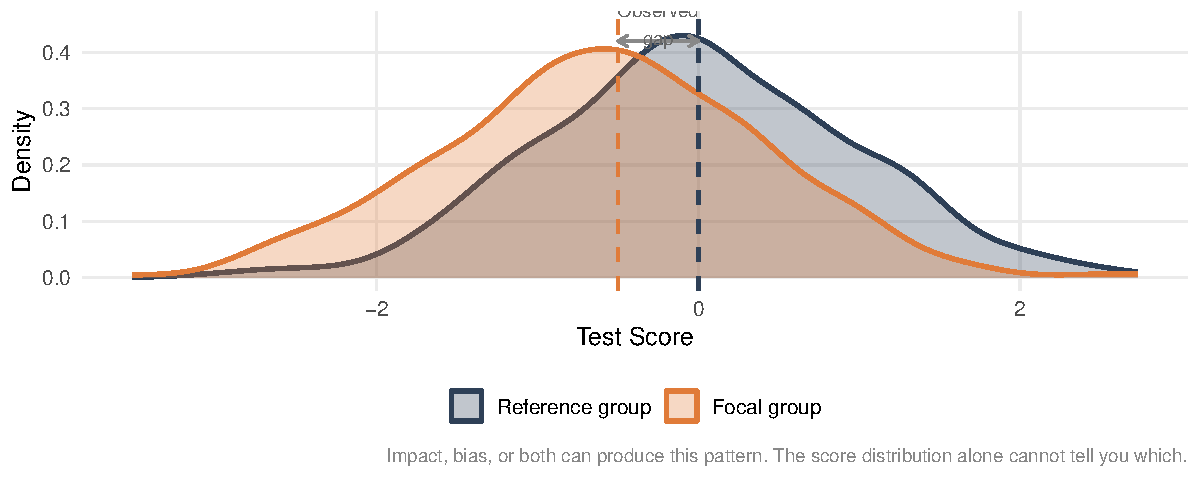
\includegraphics[width=0.85\linewidth,height=\textheight,keepaspectratio]{chapters/chapter_bias_fairness_files/figure-pdf/bias-impact-fig-1.pdf}

}

\caption{An observed group mean difference in test scores. The question
is what produces it: genuine differences in the construct (impact),
construct-irrelevant test features (bias), or both.}

\end{figure}%

\subsection{A Taxonomy of Bias
Sources}\label{a-taxonomy-of-bias-sources}

Bias can enter the measurement process at several points.
Table~\ref{tbl-bias-sources} summarizes the major sources and how each
is typically evaluated.

\begin{table}

\caption{\label{tbl-bias-sources}Sources of bias in psychological
assessment and their primary detection methods.}

\centering{

\begin{longtabu} to \linewidth {>{}l>{\raggedright}X>{\raggedright}X}
\toprule
\cellcolor[HTML]{2E4057}{\textcolor{white}{Source}} & \cellcolor[HTML]{2E4057}{\textcolor{white}{What it means}} & \cellcolor[HTML]{2E4057}{\textcolor{white}{Primary detection methods}}\\
\midrule
\textbf{Sampling} & The norming sample does not represent the target population & Demographic review of standardization sample\\
\textbf{Construct} & The construct is defined or expressed differently across groups & Multi-group CFA, measurement invariance, expert review\\
\textbf{Item} & Individual items function differently for different groups & DIF analysis (Mantel–Haenszel, logistic regression)\\
\textbf{Test-taking} & Construct-irrelevant person factors affect performance & Group comparisons, response time analysis, interviews\\
\textbf{Predictive} & The test predicts outcomes with different accuracy across groups & Differential prediction, separate regression by group\\
\bottomrule
\end{longtabu}

}

\end{table}%

These sources are not mutually exclusive. A test can show item bias and
predictive bias simultaneously, or construct bias that manifests partly
at the item level. A thorough fairness evaluation addresses multiple
sources using multiple methods. No single analysis is sufficient, and a
finding of ``no bias'' on one method does not rule out bias of other
types.

\begin{center}\rule{0.5\linewidth}{0.5pt}\end{center}

\section{Fairness Is Not a Statistic}\label{fairness-is-not-a-statistic}

Bias is a technical concept with detection methods. Fairness is
something broader.

\begin{tcolorbox}[enhanced jigsaw, colback=white, toprule=.15mm, colbacktitle=quarto-callout-note-color!10!white, left=2mm, leftrule=.75mm, opacitybacktitle=0.6, colframe=quarto-callout-note-color-frame, rightrule=.15mm, bottomtitle=1mm, opacityback=0, titlerule=0mm, toptitle=1mm, breakable, bottomrule=.15mm, coltitle=black, title=\textcolor{quarto-callout-note-color}{\faInfo}\hspace{0.5em}{Note}, arc=.35mm]

\textbf{Fairness} is a judgment about whether score-based
interpretations and uses are appropriate for specific groups in specific
contexts. It is not a fixed property of the test.

\end{tcolorbox}

This framing comes from the pragmatic tradition in measurement science,
which holds that measurement claims cannot be evaluated in the abstract.
A test is not fair or unfair in isolation. It is fair or unfair
\emph{for a purpose, with a particular group, given specific
consequences}.

The same reading comprehension test might be:

\begin{itemize}
\tightlist
\item
  Fair for native English speakers in an academic selection context
  where reading comprehension is the construct of interest
\item
  Unfair for recent immigrants in a high-stakes employment context where
  the job does not require the kind of reading comprehension the test
  measures
\item
  An open question for English language learners in an educational
  placement context, pending evidence about whether the test's
  linguistic demands are construct-relevant or construct-irrelevant for
  that use
\end{itemize}

What changes across these scenarios is not the test. It is the use, the
population, and the consequences of the decision.

This has a direct implication for how fairness claims in test manuals
and published validity studies should be evaluated. A statement like
``DIF analyses revealed no biased items'' is not a fairness conclusion.
It is one piece of evidence (item-level evidence) within a broader
argument that still needs to be made. The argument must connect the
evidence to the specific intended use, the specific population, and the
specific consequences of score-based decisions. Within Kane's (1992)
interpretation--use argument, fairness claims function as warrants. If
the warrants are not supported, the validity argument fails for that use
and that group, even if it holds for others.

Fairness review is also not a one-time event. As test uses expand to new
populations or new contexts, the evidence base must be revisited.

\begin{center}\rule{0.5\linewidth}{0.5pt}\end{center}

\section{Differential Item
Functioning}\label{differential-item-functioning}

The most widely used statistical approach to detecting item-level bias
is differential item functioning (DIF) analysis. DIF analysis asks
whether individual items on a test behave differently across groups
after accounting for overall ability or trait level.

\subsection{What DIF Is}\label{what-dif-is}

\begin{tcolorbox}[enhanced jigsaw, colback=white, toprule=.15mm, colbacktitle=quarto-callout-note-color!10!white, left=2mm, leftrule=.75mm, opacitybacktitle=0.6, colframe=quarto-callout-note-color-frame, rightrule=.15mm, bottomtitle=1mm, opacityback=0, titlerule=0mm, toptitle=1mm, breakable, bottomrule=.15mm, coltitle=black, title=\textcolor{quarto-callout-note-color}{\faInfo}\hspace{0.5em}{Note}, arc=.35mm]

An item shows \textbf{differential item functioning} when examinees from
different groups who have the same standing on the construct being
measured do not have the same probability of answering the item
correctly (or endorsing it, for Likert-type items).

\end{tcolorbox}

The key phrase is \emph{same standing on the construct}. DIF analysis is
a conditional comparison: it asks about group differences in item
performance \emph{within} ability levels, not across them. Without that
conditioning, you are measuring raw group differences in item
performance, which may simply reflect real differences in ability
(impact) rather than item malfunction.

This conditionality is what distinguishes DIF from simple item
difficulty comparisons. An item that is hard for everyone is not a
biased item. An item that is harder for one group \emph{even among
examinees who are equally able overall} is a candidate for DIF.

\subsection{The Reference/Focal Group
Structure}\label{the-referencefocal-group-structure}

DIF analyses are always comparative. You need two groups: a
\textbf{reference group} (typically the majority group or the group for
whom the test was originally developed) and a \textbf{focal group} (the
group whose item performance is being evaluated relative to the
reference group).

The choice of reference group is substantive, not statistical. It
reflects a judgment about what the comparison is for. When multiple
focal groups are of interest (e.g., by sex, race/ethnicity, and language
background), each comparison is run separately against the same
reference group. Results are not combined.

One point worth stating explicitly: DIF in either direction is a
concern. An item that statistically advantages the focal group is not
automatically acceptable. It may still contain construct-irrelevant
content that happens to benefit that group, and it warrants the same
expert review as an item that disadvantages them.

\subsection{DIF Is Neither Necessary Nor Sufficient for
Bias}\label{dif-is-neither-necessary-nor-sufficient-for-bias}

This is a conceptual point that is frequently misunderstood, including
in published research.

\textbf{DIF can exist without bias.} If an item functions differently
across groups because the groups genuinely differ on a secondary
dimension that is legitimately part of the construct, the DIF reflects
real performance differences, not measurement malfunction. Consider a
reading comprehension test that includes a passage about a scientific
concept. If students with more science background perform better on
items related to that passage, even after matching on overall reading
level, the DIF may reflect real differences in background knowledge that
are arguably part of what reading comprehension requires. Whether this
is bias or impact depends on the construct definition.

A simpler example: a scale measures weight. Men score higher than women
on average. The scale shows DIF by sex. This is not bias. It is the
scale doing its job. The construct is weight, and the groups genuinely
differ on it.

\textbf{Bias can exist without DIF.} Bias can operate at the test level
without any individual item flagging. Predictive bias (the systematic
over- or under-prediction of outcomes for a group) can exist even when
every item functions identically across groups. Construct bias, where
the construct itself is defined or experienced differently across
cultures, may not produce item-level DIF at all, because no single item
is responsible for the discrepancy. The whole instrument is misaligned.

\begin{tcolorbox}[enhanced jigsaw, colback=white, toprule=.15mm, colbacktitle=quarto-callout-important-color!10!white, left=2mm, leftrule=.75mm, opacitybacktitle=0.6, colframe=quarto-callout-important-color-frame, rightrule=.15mm, bottomtitle=1mm, opacityback=0, titlerule=0mm, toptitle=1mm, breakable, bottomrule=.15mm, coltitle=black, title=\textcolor{quarto-callout-important-color}{\faExclamation}\hspace{0.5em}{Important}, arc=.35mm]

DIF is a symptom, not a diagnosis. A flagged item is a signal that
something warrants investigation, not evidence that bias has been
confirmed. A clean DIF analysis is not evidence that no bias exists.

\end{tcolorbox}

\subsection{Uniform vs.~Non-Uniform
DIF}\label{uniform-vs.-non-uniform-dif}

DIF comes in two forms, distinguished by whether the group difference in
item performance is consistent across ability levels or varies by
ability level.

\textbf{Uniform DIF} occurs when one group consistently outperforms the
other across the entire ability range. The item is uniformly easier for
one group at every ability level. Graphically, the item characteristic
curves for the two groups are parallel but offset.

\textbf{Non-uniform DIF} occurs when the pattern of group differences
changes across ability levels. At low ability, one group may outperform
the other; at high ability, the pattern may reverse. The item
characteristic curves cross. This pattern is more complex to interpret
and has different implications for the choice of detection method.

\begin{figure}[H]

{\centering 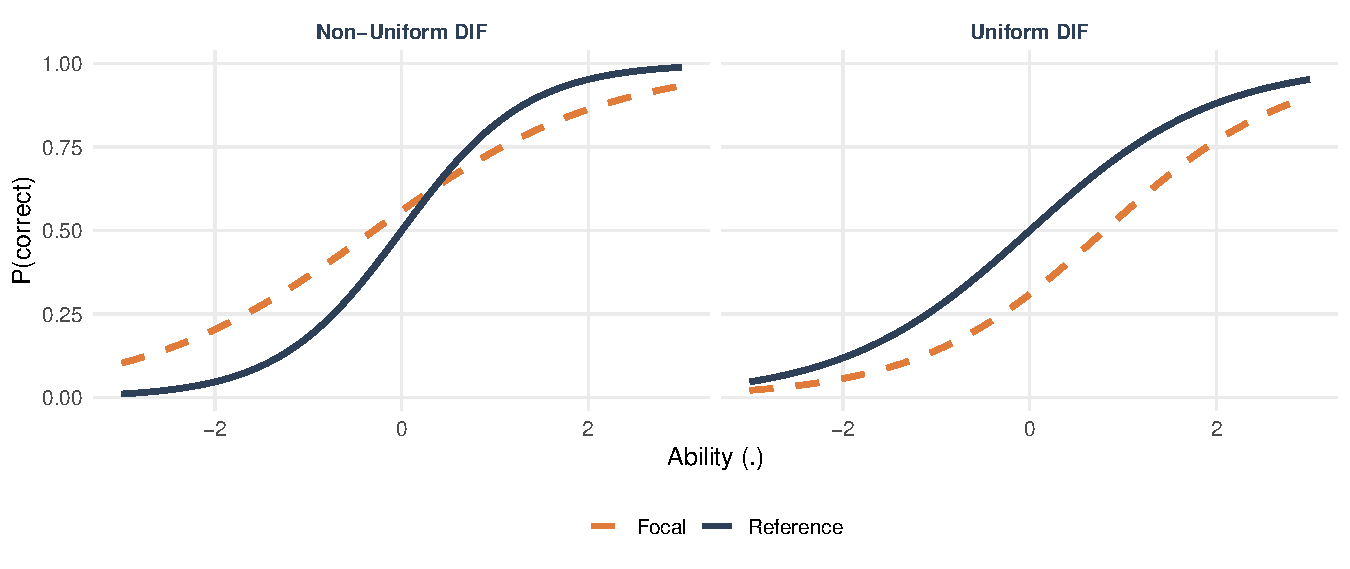
\includegraphics[width=0.85\linewidth,height=\textheight,keepaspectratio]{chapters/chapter_bias_fairness_files/figure-pdf/uniform-nonuniform-fig-1.pdf}

}

\caption{Uniform DIF (left): one group consistently outperforms the
other at all ability levels. Non-uniform DIF (right): the group
difference changes direction across ability levels. MH detects uniform
DIF only; logistic regression detects both.}

\end{figure}%

\begin{center}\rule{0.5\linewidth}{0.5pt}\end{center}

\section{Classical DIF Methods}\label{classical-dif-methods}

Two classical (non-IRT) methods dominate applied DIF analysis: the
Mantel--Haenszel procedure and logistic regression. Both condition on
total test score as a proxy for ability. Both are available in R through
the \texttt{difR} package (Magis et al., 2010).

\subsection{The Mantel--Haenszel
Procedure}\label{the-mantelhaenszel-procedure}

The Mantel--Haenszel (MH) procedure (Holland \& Thayer, 1986) was
developed at Educational Testing Service and became the dominant method
for large-scale DIF detection. Its prevalence in applied testing
reflects historical adoption and practical interpretability more than
statistical superiority, a point we return to below.

\textbf{Logic.} MH stratifies examinees by their total test score.
Within each score stratum, it constructs a 2×2 table: group membership
(reference vs.~focal) × item response (correct vs.~incorrect). It then
combines these stratum-specific tables into a summary statistic that
tests whether the odds of correct response differ by group after
conditioning on ability.

Within a single stratum, the comparison looks like this:

\begin{longtable*}[t]{lccc}
\toprule
\cellcolor[HTML]{2E4057}{\textcolor{white}{Group}} & \cellcolor[HTML]{2E4057}{\textcolor{white}{Correct}} & \cellcolor[HTML]{2E4057}{\textcolor{white}{Incorrect}} & \cellcolor[HTML]{2E4057}{\textcolor{white}{P(correct)}}\\
\midrule
Reference & 28 & 12 & .70\\
Focal & 16 & 14 & .53\\
\bottomrule
\end{longtable*}

If the focal group consistently shows lower correct-response rates
across strata (after conditioning on total score), MH will detect it.

\textbf{Key output.}

\begin{longtable}[t]{lccccc}

\caption{\label{tbl-mh-results}Mantel--Haenszel DIF results for the
15-item reading comprehension dataset. Items flagged at Class B or C are
candidates for substantive review.}

\tabularnewline

\toprule
\cellcolor[HTML]{2E4057}{\textcolor{white}{Item}} & \cellcolor[HTML]{2E4057}{\textcolor{white}{MH χ²}} & \cellcolor[HTML]{2E4057}{\textcolor{white}{p}} & \cellcolor[HTML]{2E4057}{\textcolor{white}{MH Δ}} & \cellcolor[HTML]{2E4057}{\textcolor{white}{ETS Class}} & \cellcolor[HTML]{2E4057}{\textcolor{white}{Flag}}\\
\midrule
Item 1 & 2.04 & 0.154 & -0.91 & A & \\
Item 2 & 0.03 & 0.861 & 0.16 & A & \\
\cellcolor[HTML]{FFF2CC}{Item 3} & \cellcolor[HTML]{FFF2CC}{5.51} & \cellcolor[HTML]{FFF2CC}{0.019} & \cellcolor[HTML]{FFF2CC}{-1.34} & \cellcolor[HTML]{FFF2CC}{B} & \cellcolor[HTML]{FFF2CC}{! Moderate}\\
Item 4 & 1.13 & 0.288 & 0.68 & A & \\
Item 5 & 0.18 & 0.675 & -0.30 & A & \\
\addlinespace
Item 6 & 0.02 & 0.886 & 0.14 & A & \\
Item 7 & 3.15 & 0.076 & -1.12 & A & \\
Item 8 & 0.21 & 0.646 & -0.29 & A & \\
Item 9 & 0.01 & 0.941 & 0.10 & A & \\
\cellcolor[HTML]{FCE4D6}{Item 10} & \cellcolor[HTML]{FCE4D6}{15.31} & \cellcolor[HTML]{FCE4D6}{0.000} & \cellcolor[HTML]{FCE4D6}{2.29} & \cellcolor[HTML]{FCE4D6}{C} & \cellcolor[HTML]{FCE4D6}{!! Large}\\
\addlinespace
Item 11 & 0.00 & 0.991 & 0.07 & A & \\
Item 12 & 0.84 & 0.358 & -0.53 & A & \\
Item 13 & 0.69 & 0.406 & 0.52 & A & \\
Item 14 & 0.13 & 0.719 & 0.28 & A & \\
Item 15 & 0.14 & 0.711 & 0.27 & A & \\
\bottomrule

\end{longtable}

Three statistics matter:

\begin{itemize}
\tightlist
\item
  \textbf{MH χ²} tests whether item performance differs by group after
  conditioning on total score. A significant result indicates DIF is
  present.
\item
  \textbf{MH Δ (delta)} is the effect size. A negative delta means the
  item is easier for the focal group; a positive delta means it is
  easier for the reference group. The magnitude determines the ETS
  classification regardless of direction.
\item
  \textbf{ETS classification} (A, B, or C) provides a practical severity
  rating. Class A indicates negligible DIF with no action required.
  Class B indicates moderate DIF warranting expert review. Class C
  indicates large DIF; the item should not be retained without
  substantive review.
\end{itemize}

The thresholds are: \textbar Δ\textbar{} must be ≥ 1.0 \emph{and} the
result must be statistically significant to leave Class A.
\textbar Δ\textbar{} ≥ 1.5 \emph{and} statistical significance places an
item in Class C.

\textbf{What MH cannot do.} MH detects uniform DIF only. It cannot
detect non-uniform DIF, meaning patterns where the group difference
changes across ability levels. It also assumes the total score is a
clean proxy for ability, which becomes problematic if biased items are
included in the total score (the purification problem, discussed below).

\subsubsection{Running the Mantel--Haenszel Procedure in
R}\label{running-the-mantelhaenszel-procedure-in-r}

The \texttt{difMH()} function in the \texttt{difR} package runs the full
MH procedure. The three required inputs are the item response matrix, a
group vector, and a matching variable (typically the total score).

\begin{Shaded}
\begin{Highlighting}[]
\FunctionTok{library}\NormalTok{(difR)}

\CommentTok{\# Item responses only (no id or group column)}
\NormalTok{items }\OtherTok{\textless{}{-}}\NormalTok{ dat[, }\FunctionTok{paste0}\NormalTok{(}\StringTok{"item"}\NormalTok{, }\DecValTok{1}\SpecialCharTok{:}\DecValTok{15}\NormalTok{)]}

\CommentTok{\# Group vector (0 = reference, 1 = focal)}
\NormalTok{group }\OtherTok{\textless{}{-}}\NormalTok{ dat}\SpecialCharTok{$}\NormalTok{group}

\CommentTok{\# Total score as matching variable}
\NormalTok{total }\OtherTok{\textless{}{-}} \FunctionTok{rowSums}\NormalTok{(items)}

\CommentTok{\# Run MH DIF analysis}
\NormalTok{mh\_result }\OtherTok{\textless{}{-}} \FunctionTok{difMH}\NormalTok{(}
  \AttributeTok{Data       =}\NormalTok{ items,}
  \AttributeTok{group      =}\NormalTok{ group,}
  \AttributeTok{focal.name =} \DecValTok{1}\NormalTok{,}
  \AttributeTok{match      =}\NormalTok{ total,}
  \AttributeTok{correct    =} \ConstantTok{TRUE}\NormalTok{,   }\CommentTok{\# Yates continuity correction}
  \AttributeTok{alpha      =} \FloatTok{0.05}
\NormalTok{)}

\CommentTok{\# View results}
\FunctionTok{print}\NormalTok{(mh\_result)}
\end{Highlighting}
\end{Shaded}

The \texttt{focal.name\ =\ 1} argument tells \texttt{difMH} which value
in the group vector identifies the focal group. The
\texttt{correct\ =\ TRUE} argument applies a continuity correction to
the chi-square statistic, which is recommended for small cell sizes.
Setting \texttt{purify\ =\ TRUE} would run the iterative purification
procedure described above; the default is \texttt{FALSE}.

Output includes the MH chi-square, p-value, and alpha (the odds ratio)
for each item. The delta and ETS classification are derived from the
alpha as shown in the results table above. If you need to inspect the
raw slot names in your version of \texttt{difR}, run
\texttt{names(mh\_result)} after fitting the model.

\subsection{Logistic Regression DIF}\label{logistic-regression-dif}

Logistic regression DIF (Swaminathan \& Rogers, 1990) extends MH by
modeling the probability of correct response as a function of total
score, group membership, and their interaction. It is statistically more
capable than MH and is the recommended method when software is
available.

Three nested models are estimated for each item:

\begin{table}

\caption{\label{tbl-lr-models}The three nested logistic regression
models used in LR DIF analysis.}

\centering{

\begin{longtabu} to \linewidth {>{}l>{\raggedright}X>{\raggedright}X}
\toprule
\cellcolor[HTML]{2E4057}{\textcolor{white}{Model}} & \cellcolor[HTML]{2E4057}{\textcolor{white}{Predictors}} & \cellcolor[HTML]{2E4057}{\textcolor{white}{What it tests}}\\
\midrule
\textbf{Model 1} & Total score & Baseline — ability predicts item response\\
\textbf{Model 2} & Total score + group & Uniform DIF — group predicts response after controlling for ability\\
\textbf{Model 3} & Total score + group + group × score & Non-uniform DIF — group effect varies by ability level\\
\bottomrule
\end{longtabu}

}

\end{table}%

Uniform DIF is indicated by a significant improvement from Model 1 to
Model 2 (significant group term). Non-uniform DIF is indicated by a
significant improvement from Model 2 to Model 3 (significant interaction
term). Effect size is evaluated using R² change alongside the
significance tests. A statistically significant finding with a very
small R² change may not be practically meaningful, especially in large
samples.

\begin{longtable}[t]{lcccc}

\caption{\label{tbl-lr-results}Logistic regression DIF results for
flagged items. The interaction term tests for non-uniform DIF, which MH
cannot detect.}

\tabularnewline

\toprule
\cellcolor[HTML]{2E4057}{\textcolor{white}{Item}} & \cellcolor[HTML]{2E4057}{\textcolor{white}{Group term p}} & \cellcolor[HTML]{2E4057}{\textcolor{white}{Interaction p}} & \cellcolor[HTML]{2E4057}{\textcolor{white}{R² change}} & \cellcolor[HTML]{2E4057}{\textcolor{white}{DIF type}}\\
\midrule
Item 3 & .009 & .44 & .018 & Uniform\\
Item 5 & <.001 & .38 & .041 & Uniform\\
Item 7 & .03 & .41 & .015 & Uniform\\
\cellcolor[HTML]{FFF2CC}{Item 9} & \cellcolor[HTML]{FFF2CC}{.004} & \cellcolor[HTML]{FFF2CC}{.02} & \cellcolor[HTML]{FFF2CC}{.031} & \cellcolor[HTML]{FFF2CC}{Non-uniform}\\
Item 10 & .13 & .61 & .009 & —\\
\addlinespace
Item 13 & .02 & .55 & .012 & Uniform\\
\bottomrule

\end{longtable}

The results for Item 9 are instructive. MH classified it as Class C with
Δ = −1.6, suggesting large uniform DIF favoring the focal group. The
logistic regression interaction term is significant (\emph{p} = .02),
revealing that the pattern is actually non-uniform: the group difference
in item performance changes across ability levels. MH averaged over this
crossing pattern and reported it as a consistent direction of DIF, which
is misleading. Logistic regression reveals the more complex picture.

\textbf{Why MH is still widely used.} If logistic regression is more
capable, why does MH dominate applied testing? The answer is historical
and practical, not statistical. MH was developed at ETS decades before
logistic regression DIF became standard, and its delta metric and A/B/C
classification system became embedded in testing practice. Most
published test manuals report MH results. The multiplicity concern (that
running many significance tests inflates Type I error) applies equally
to both methods, so it is not a reason to prefer MH. When logistic
regression is available, it should be used. When reading applied
reports, MH results need to be understood and evaluated critically.

\subsection{The Purification Problem}\label{the-purification-problem}

Both MH and logistic regression use the total test score as the matching
variable, the proxy for ability that conditioning is done on. This
creates a circularity: if some items are biased against the focal group,
those students earn lower total scores, which means they get matched
against lower-ability reference group members in the strata. True DIF on
some items may be masked; spurious DIF may appear on others.

The standard solution is \textbf{purification}: an iterative procedure
in which flagged items are removed from the matching variable and the
analysis is re-run on the remaining items. This continues until the set
of flagged items stabilizes. Purification is implemented in
\texttt{difR} via the \texttt{purify\ =\ TRUE} argument.

In practice, purification rarely changes conclusions dramatically unless
the test is short or heavily biased. It is nonetheless worth conducting
as a sensitivity check, particularly when a large proportion of items
are flagged.

\subsection{From Statistical Flag to Substantive
Judgment}\label{from-statistical-flag-to-substantive-judgment}

A DIF flag is not a bias determination. It is an invitation to
investigate. The statistical result tells you that an item is behaving
differently after conditioning on ability; it does not tell you why.

An item can be flagged because:

\begin{itemize}
\tightlist
\item
  It contains construct-irrelevant content that systematically
  disadvantages the focal group. This is bias, and the item should be
  revised or removed.
\item
  It taps a secondary dimension on which the groups legitimately differ.
  This is impact, and the item may be retained depending on the
  construct definition.
\item
  It uses vocabulary or cultural context that is more familiar to the
  reference group. This may be bias, and requires expert evaluation of
  whether that familiarity is construct-relevant.
\item
  The matching variable is contaminated by other biased items. This is a
  methodological artifact that purification can address.
\end{itemize}

Resolving the ambiguity requires substantive expert review: people with
knowledge of the construct, the groups involved, and the cultural and
linguistic context of the items. The statistics open the conversation.
Expert judgment closes it.

\textbf{Returning to Item 7.} Recall the item introduced in the lecture
slides: \emph{``Which word best completes the sentence: `The scientist's
findings were met with widespread \_\_\_\_\_ from the academic
community.'\,''} Suppose this item flags as Class C uniform DIF favoring
the reference group (majority English speakers). Does that mean it is
biased?

Not necessarily. ELL students may perform worse on this item because
vocabulary breadth (including academic English vocabulary) legitimately
differs between the groups and is arguably part of reading
comprehension. That is impact. But if the item is on a test of
scientific reasoning rather than vocabulary, and ``acclaim'' is not the
kind of word that scientific reasoning requires, then the vocabulary
demand is construct-irrelevant. That is bias. The statistics cannot
distinguish these explanations. A reading specialist and an ELL
education expert reviewing the item together can.

\begin{center}\rule{0.5\linewidth}{0.5pt}\end{center}

\section{Measurement Invariance}\label{measurement-invariance}

DIF analysis operates at the item level. Measurement invariance operates
at the factor level. Both address the same fundamental question: do
scores mean the same thing across groups? They differ only in the level
of the measurement model at which they operate.

\subsection{A Brief Recap}\label{a-brief-recap}

As covered in Chapters 7 and 8, confirmatory factor analysis (CFA)
models the relationship between observed items and one or more latent
factors. Measurement invariance testing uses multi-group CFA to evaluate
whether that model holds up across groups.

Three levels of invariance are typically assessed:

\textbf{Configural invariance} means the same factor structure (which
items load on which factors) holds across groups. This is the weakest
form and is a precondition for the others.

\textbf{Metric invariance} (weak invariance) means factor loadings are
equal across groups. Equal loadings mean that the relationship between
the latent factor and the observed items is the same for both groups;
the items are measuring the construct with the same sensitivity.

\textbf{Scalar invariance} (strong invariance) means factor loadings and
item intercepts are equal across groups. Equal intercepts mean that at
the same level of the latent factor, the expected item scores are the
same for both groups. This is required for meaningful comparison of
latent means across groups.

When scalar invariance holds, group mean differences in observed scores
can be interpreted as group mean differences in the latent construct.
The scores are measuring the same thing in the same way, with the same
scale origin. When it fails, observed score differences are contaminated
by differences in item intercepts, and latent mean comparisons cannot be
made without qualification.

\subsection{Invariance and DIF Are Two Levels of the Same
Question}\label{invariance-and-dif-are-two-levels-of-the-same-question}

The conceptual link between DIF and measurement invariance is direct.
DIF at the item level and non-invariance at the factor level are
manifestations of the same underlying problem: the measurement model
does not hold equally across groups.

Non-invariant intercepts at the CFA level correspond to uniform DIF at
the item level. Items with different intercepts across groups are items
that are systematically easier or harder for one group after accounting
for the latent factor, which is exactly what MH and logistic regression
detect. Non-invariant loadings correspond to a form of non-uniform DIF
in which the sensitivity of the item to the construct differs by group.

When both DIF and invariance analyses are available, they should be
interpreted together. A finding of metric but not scalar invariance,
combined with several Class C DIF items, tells a consistent story about
where the measurement model breaks down.

\subsection{Partial Invariance}\label{partial-invariance}

Full scalar invariance is frequently not achieved in practice,
particularly across groups with substantial cultural or linguistic
differences. \textbf{Partial invariance}, where some but not all items
show invariant intercepts, permits limited comparisons if the
non-invariant items are identified and handled appropriately.

With partial invariance, latent mean comparisons are possible if at
least two items per factor show invariant intercepts (to anchor the
scale). The non-invariant items are freed across groups in the model,
and their contribution to the comparison is explicitly accounted for.
This is a more defensible position than either assuming full invariance
when it does not hold or abandoning cross-group comparisons entirely.

The practical implication: a finding of partial scalar invariance should
prompt the same substantive review process as a DIF flag. Which items
are non-invariant? What do they have in common? Is there a substantive
explanation (cultural specificity, linguistic complexity, content
familiarity) that suggests construct-irrelevant variance?

\subsection{Running an Invariance Test in
R}\label{running-an-invariance-test-in-r}

Measurement invariance testing uses the \texttt{lavaan} package, which
was introduced in Chapters 7 and 8. The abbreviated workflow is:

\begin{Shaded}
\begin{Highlighting}[]
\FunctionTok{library}\NormalTok{(lavaan)}

\CommentTok{\# Specify the model (example: single factor, 5 items)}
\NormalTok{model }\OtherTok{\textless{}{-}} \StringTok{\textquotesingle{}}
\StringTok{  factor1 =\textasciitilde{} item1 + item2 + item3 + item4 + item5}
\StringTok{\textquotesingle{}}

\CommentTok{\# Configural: same structure, all parameters free}
\NormalTok{fit\_config }\OtherTok{\textless{}{-}} \FunctionTok{cfa}\NormalTok{(model, }\AttributeTok{data =}\NormalTok{ dat, }\AttributeTok{group =} \StringTok{"group"}\NormalTok{)}

\CommentTok{\# Metric: constrain loadings equal}
\NormalTok{fit\_metric }\OtherTok{\textless{}{-}} \FunctionTok{cfa}\NormalTok{(model, }\AttributeTok{data =}\NormalTok{ dat, }\AttributeTok{group =} \StringTok{"group"}\NormalTok{,}
                  \AttributeTok{group.equal =} \StringTok{"loadings"}\NormalTok{)}

\CommentTok{\# Scalar: constrain loadings and intercepts equal}
\NormalTok{fit\_scalar }\OtherTok{\textless{}{-}} \FunctionTok{cfa}\NormalTok{(model, }\AttributeTok{data =}\NormalTok{ dat, }\AttributeTok{group =} \StringTok{"group"}\NormalTok{,}
                  \AttributeTok{group.equal =} \FunctionTok{c}\NormalTok{(}\StringTok{"loadings"}\NormalTok{, }\StringTok{"intercepts"}\NormalTok{))}

\CommentTok{\# Compare models}
\FunctionTok{lavTestLRT}\NormalTok{(fit\_config, fit\_metric, fit\_scalar)}
\end{Highlighting}
\end{Shaded}

A significant chi-square difference test between the metric and scalar
models indicates that at least one intercept is non-invariant.
Modification indices identify which items are responsible. The
\texttt{lavTestScore()} function provides item-level detail on where the
model is misspecified.

Fit index changes alongside chi-square tests provide additional
guidance: a ΔCFI of less than −0.010 and ΔRMSEA of less than 0.015
suggest acceptable invariance even when the chi-square difference is
significant, particularly in large samples where the test is sensitive
to trivial misfit (Cheung \& Rensvold, 1999).

\begin{center}\rule{0.5\linewidth}{0.5pt}\end{center}

\section{Predictive Bias}\label{predictive-bias}

Item-level DIF and measurement invariance address whether the test
measures the construct equivalently across groups. Predictive bias
addresses a different question: whether the test predicts outcomes with
equal accuracy across groups.

\begin{tcolorbox}[enhanced jigsaw, colback=white, toprule=.15mm, colbacktitle=quarto-callout-note-color!10!white, left=2mm, leftrule=.75mm, opacitybacktitle=0.6, colframe=quarto-callout-note-color-frame, rightrule=.15mm, bottomtitle=1mm, opacityback=0, titlerule=0mm, toptitle=1mm, breakable, bottomrule=.15mm, coltitle=black, title=\textcolor{quarto-callout-note-color}{\faInfo}\hspace{0.5em}{Note}, arc=.35mm]

\textbf{Predictive bias} occurs when a test systematically over- or
under-predicts a criterion outcome for members of one group, relative to
what would be predicted on the basis of ability alone.

\end{tcolorbox}

The distinction is important. A test can show no item-level DIF, full
measurement invariance, and still show predictive bias. These analyses
address different aspects of measurement and use. A complete fairness
argument requires attention to all of them.

\subsection{Detecting Predictive Bias}\label{detecting-predictive-bias}

Predictive bias is evaluated by fitting separate regression lines
predicting the criterion (e.g., GPA, job performance, diagnosis) from
test scores for each group. Three patterns are possible:

\textbf{No predictive bias:} slopes and intercepts are equal. The test
predicts the criterion equally well for both groups, with no systematic
over- or under-prediction.

\textbf{Slope differences:} the test is more predictive for one group
than the other. The regression lines converge or diverge across the
score range. This is non-uniform predictive bias, where the prediction
error varies depending on where in the score distribution an examinee
falls.

\textbf{Intercept differences with equal slopes:} the most common
pattern. The test predicts with equal accuracy for both groups (similar
slopes and correlations), but systematically over- or under-predicts for
one group at every score level.

\begin{figure}[H]

{\centering 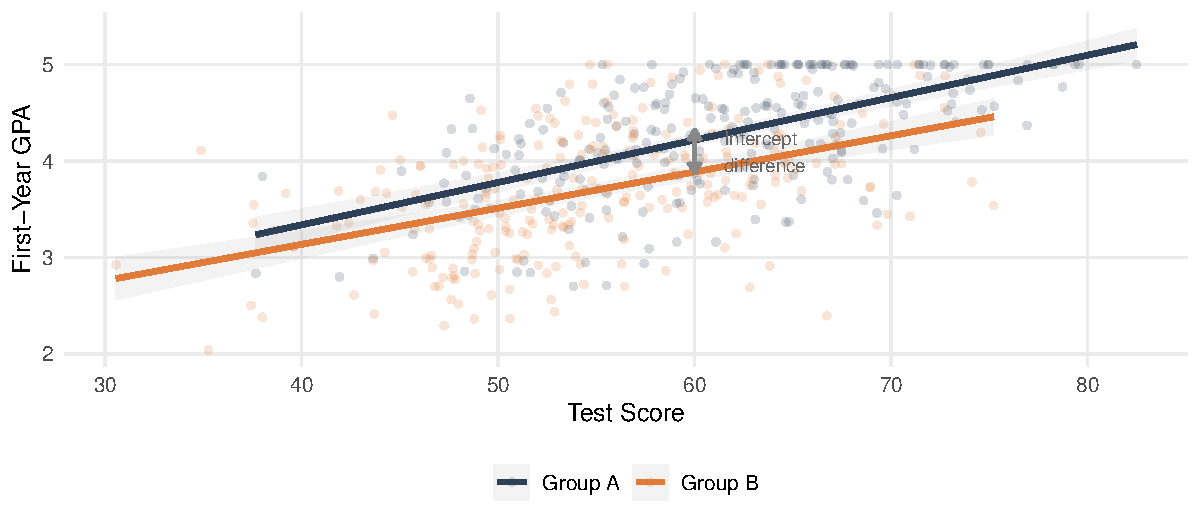
\includegraphics[width=0.85\linewidth,height=\textheight,keepaspectratio]{chapters/chapter_bias_fairness_files/figure-pdf/pred-bias-fig-1.pdf}

}

\caption{Differential prediction with equal slopes but different
intercepts. The test predicts GPA with similar accuracy for both groups,
but systematically underpredicts actual GPA for Group B at every score
level.}

\end{figure}%

The intercept difference pattern is particularly consequential in
high-stakes contexts. When slopes are equal, the test is equally
\emph{predictive} for both groups: both regression lines have the same
relationship between score and outcome. But the intercept gap means the
test score is used to make decisions that systematically misclassify
members of one group. A Group B candidate with the same test score as a
Group A candidate is predicted to perform worse, but if intercepts
differ, that prediction is systematically wrong. The test undersells
Group B.

In the special education context: if a cognitive assessment
systematically underpredicts the academic performance of children from
certain linguistic or cultural backgrounds, eligibility determinations
based on that assessment will systematically exclude children who would
benefit from services, and include others who would not. The error is
not random; it is directional and group-specific.

\begin{center}\rule{0.5\linewidth}{0.5pt}\end{center}

\section{Accumulating a Fairness
Argument}\label{accumulating-a-fairness-argument}

No single analysis constitutes a fairness conclusion. A well-supported
fairness argument draws on multiple sources of evidence, each addressing
a different aspect of the question.

\begin{table}

\caption{\label{tbl-fairness-evidence}Sources of evidence in a fairness
argument. Each addresses a different aspect of measurement equivalence
and appropriate use.}

\centering{

\begin{longtabu} to \linewidth {>{}l>{\raggedright}X>{\raggedright}X}
\toprule
\cellcolor[HTML]{2E4057}{\textcolor{white}{Evidence}} & \cellcolor[HTML]{2E4057}{\textcolor{white}{What it addresses}} & \cellcolor[HTML]{2E4057}{\textcolor{white}{Method}}\\
\midrule
\textbf{Item-level DIF} & Individual items functioning differently across groups & MH, logistic regression DIF\\
\textbf{Measurement invariance} & Construct equivalence at the factor level & Multi-group CFA\\
\textbf{Predictive validity} & Equal accuracy and absence of systematic bias in prediction & Differential prediction, separate regression by group\\
\textbf{Norm sample adequacy} & Norm sample representing the target population & Demographic review\\
\textbf{Qualitative review} & Sources of bias not detectable by statistics & Cognitive interviews, expert panels, focus groups\\
\bottomrule
\end{longtabu}

}

\end{table}%

When evaluating a test manual or published validity study, the relevant
questions are:

\begin{itemize}
\tightlist
\item
  Were DIF analyses conducted? Which method? Were results reported
  transparently, with full output rather than just a summary statement?
\item
  Were flagged items reviewed substantively, or simply removed? Was the
  rationale documented?
\item
  Was measurement invariance tested? At what levels? Was partial
  invariance acknowledged and addressed?
\item
  Was predictive validity examined by group? Were slope and intercept
  differences tested?
\item
  Was the norming sample appropriate for the population with whom the
  test is being used?
\item
  Did the authors distinguish between statistical DIF and substantive
  bias? Between impact and bias?
\item
  Were fairness claims commensurate with the evidence presented?
\end{itemize}

A statement like ``no items were flagged for DIF'' does not answer most
of these questions. It answers one of them.

\begin{center}\rule{0.5\linewidth}{0.5pt}\end{center}

\section{A Note on IRT-Based DIF}\label{a-note-on-irt-based-dif}

The methods covered in this chapter (MH and logistic regression) are
\emph{classical} DIF methods. They use the total test score as a proxy
for the underlying ability or trait. This proxy is imperfect: the total
score is computed from all items, including any that may be biased,
which can contaminate the matching variable and attenuate DIF estimates.

Item Response Theory (IRT) offers a more principled approach. IRT models
the relationship between examinees' latent trait levels and their item
responses directly, producing ability estimates that can be based on
non-flagged items only. IRT-based DIF methods condition on these
estimated ability parameters rather than on the total score, removing
much of the circularity that plagues classical approaches.

The conceptual question is identical: do examinees from different groups
who have the same latent trait level respond differently to this item?
What changes is the precision and cleanliness of the ability estimate
used to answer it.

IRT-based DIF is not covered in this chapter because it requires a
foundation in IRT that has not yet been established. Chapter 13
introduces IRT as a measurement framework and revisits DIF from an IRT
perspective, including a discussion of when IRT-based methods are worth
the additional complexity and when classical methods are adequate.

\begin{center}\rule{0.5\linewidth}{0.5pt}\end{center}

\section{Summary}\label{summary}

This chapter has addressed the question of whether scores mean the same
thing across groups: at the item level, at the factor level, and at the
level of score use.

The key points:

\begin{itemize}
\tightlist
\item
  \textbf{Bias} is systematic, construct-irrelevant variance that
  differentially affects scores across groups. It is a property of the
  measurement instrument, not of the test takers.
\item
  \textbf{Impact} refers to group differences that reflect genuine
  differences on the construct. The same observed score gap can reflect
  bias, impact, or both. Statistics cannot distinguish them without
  substantive judgment.
\item
  \textbf{Fairness} is a judgment about whether score-based
  interpretations and uses are appropriate for specific groups in
  specific contexts. It is not a property of the test and cannot be
  established by any single analysis.
\item
  \textbf{DIF analysis} detects item-level differential functioning
  after conditioning on ability. MH detects uniform DIF; logistic
  regression detects both uniform and non-uniform DIF. A DIF flag opens
  an investigation; expert review closes it.
\item
  \textbf{DIF is neither necessary nor sufficient for bias.} DIF can
  exist without bias (impact); bias can exist without DIF (predictive
  bias, construct bias).
\item
  \textbf{Measurement invariance} tests whether the factor model holds
  equivalently across groups. Non-invariant intercepts correspond to
  item-level DIF; both reflect the same underlying problem at different
  levels of analysis.
\item
  \textbf{Predictive bias} addresses whether scores forecast outcomes
  with equal accuracy across groups. A test can show no item-level DIF
  and still show predictive bias.
\item
  A complete \textbf{fairness argument} draws on all of these sources of
  evidence, connects them to the specific intended use and population,
  and is explicit about what the evidence does and does not establish.
\end{itemize}

\chapter{}\label{section-8}

\chapter{}\label{section-9}

\part{Evaluation and Integration}

\chapter{}\label{section-10}

\chapter{}\label{section-11}

\bookmarksetup{startatroot}

\chapter*{References}\label{references}
\addcontentsline{toc}{chapter}{References}

\markboth{References}{References}

\phantomsection\label{refs}
\begin{CSLReferences}{1}{0}
\bibitem[\citeproctext]{ref-cheung1999}
Cheung, G. W., \& Rensvold, R. B. (1999). Testing factorial invariance
across groups: A reconceptualization and proposed new method.
\emph{Journal of Management}, \emph{25}(1), 1--27.
\url{https://doi.org/10.1177/014920639902500101}

\bibitem[\citeproctext]{ref-holland1986}
Holland, P. W., \& Thayer, D. T. (1986). \emph{Differential item
performance and the {Mantel-Haenszel} procedure}. 129--145.

\bibitem[\citeproctext]{ref-kane1992}
Kane, M. T. (1992). An argument-based approach to validity.
\emph{Psychological Bulletin}, \emph{112}(3), 527--535.
\url{https://doi.org/10.1037/0033-2909.112.3.527}

\bibitem[\citeproctext]{ref-magis2010}
Magis, D., Béland, S., Tuerlinckx, F., \& De Boeck, P. (2010). A general
framework and an {R} package for the detection of dichotomous
differential item functioning. \emph{Behavior Research Methods},
\emph{42}(3), 847--862. \url{https://doi.org/10.3758/BRM.42.3.847}

\bibitem[\citeproctext]{ref-swaminathan1990}
Swaminathan, H., \& Rogers, H. J. (1990). Detecting differential item
functioning using logistic regression procedures. \emph{Journal of
Educational Measurement}, \emph{27}(4), 361--370.
\url{https://doi.org/10.1111/j.1745-3984.1990.tb00754.x}

\end{CSLReferences}


\backmatter


\end{document}
